\chapter{VANS macroscopic applications}

\chapquote{I had to make some optimistic assumptions to meet the revenue target. In week three, we’re visited by an alien named Dutox Inag who offers to share his advanced technology.}{}{Dilbert comics by Scott Adams}

\section{Introduction}

In the last chapter the macroscopic VANS equation are validated against the full microscopic DNS in a reference case. Also the permeability tensor metamodel is introduced in the algorithm to asserts its usability and correctness. The computation is performed in two different configurations, the closed cavity and the periodic hill case. The aim for the cavity problem is to validate the VANS approach and show the importance of the permeability metamodel. The periodic hill case instead served us to test the performance of porous coating as a device that helps to reduce naturally separated flow.


\section{Closed cavity}
The problem we want to solve is the classical closed cavity in two dimensions.
The cavity is a square with size $L$, the lateral and bottom walls are fixed and a constant velocity $U^{top}$ is specified at the top side.
On the front and back side we apply periodic boundary condition since the simulation domain has a depth equal to $\ell$.
A rigid porous media made by fibers is present at the bottom of the cavity and has vertical extension equal to $h$.
The \textit{reference elementary volume} of the porous medium is a cubic cell of size $\ell$ with a cylinder with diameter $d$ at his center (regular arrangement of the fibers).
The permeability of the medium $\varepsilon$ is equal to 0.8 and the microscopic length scale has been chosen in order to have 50 fibers in the cavity.

\begin{figure}[h]
\centering
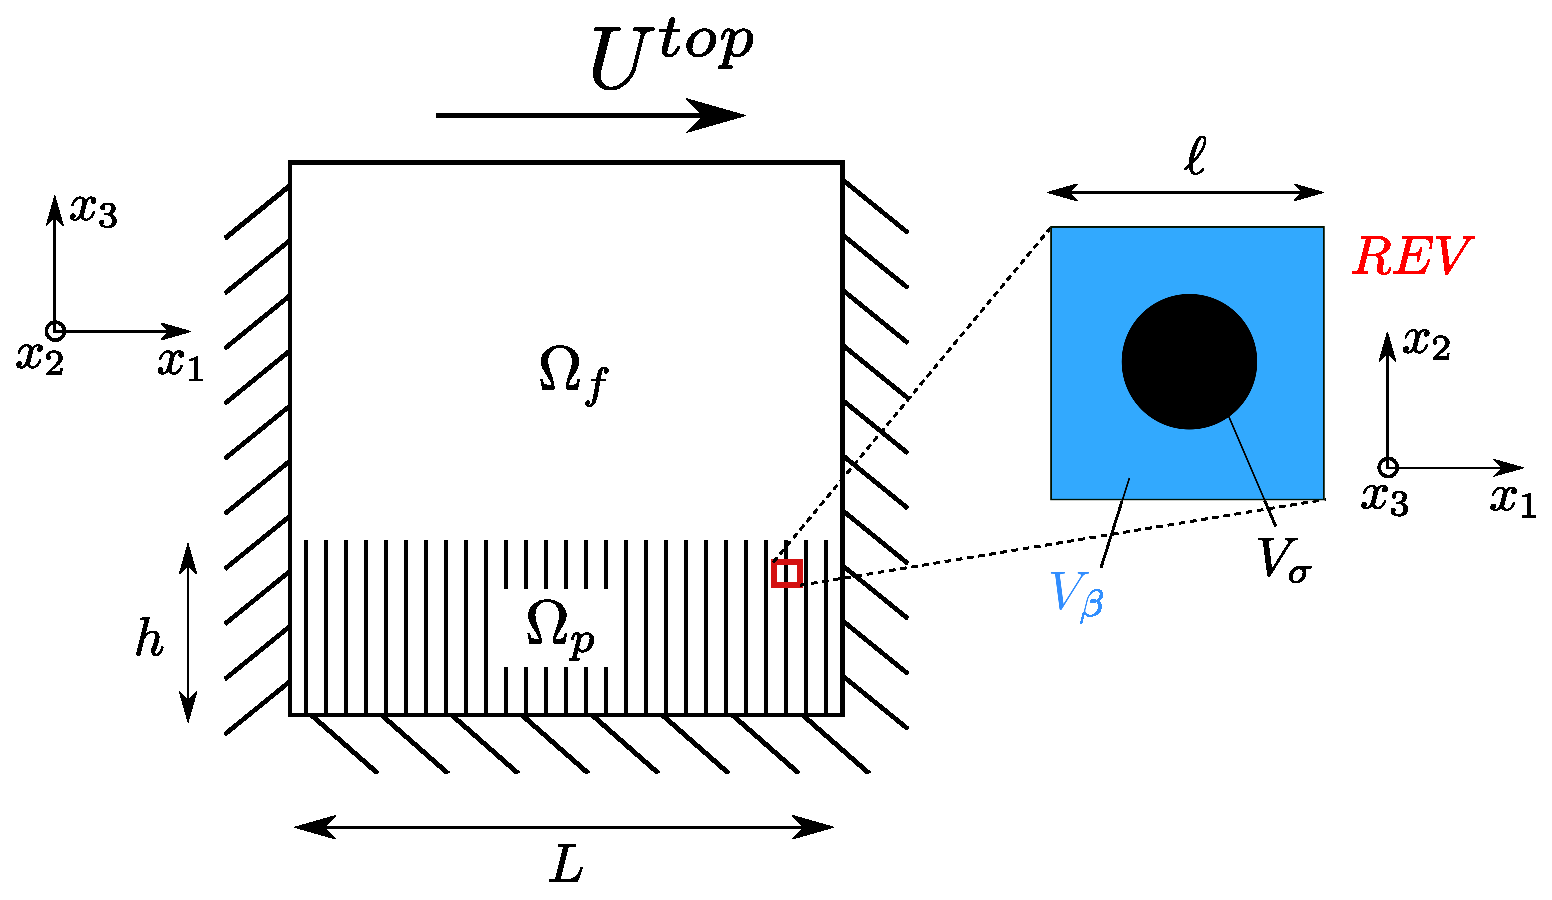
\includegraphics[width=0.7\linewidth]{chapter_5/figure/cavity_draw.eps}
\caption{Schematics of the closed cavity 2D problem. The porous medium internal structure is depicted in the zoom on the right side in which the REV geometry is showed.}
\label{fig:geom}
\end{figure}

To summarize the configuration:
\begin{itemize}
	\item $L$: side of the cavity, also the macroscopic length scale
	\item $h$: vertical extension of the fibers from the bottom of the cavity 
	\item $\ell$: side of the cubic REV, also the microscopic length scale
	\item $d$: diameter of the cylindrical fiber
	\item $V_{\beta}$: volume of the fluid inside the REV
	\item $V_{\sigma}$: volume of the solid inside the REV
	\item $\varepsilon = \dfrac{V_{\beta}}{V_{\sigma} +V_{\beta}}$: porosity of the medium
	\item $\epsilon = \dfrac{\ell}{L}$: length scale ratio
	\item $Re= \dfrac{U^{top} L}{\nub}$: Reynolds number of the cavity
\end{itemize}

The overall domain has the size $L \, \times \, L \times \, \ell$ respectively in the $x_1$, $x_2$ and $x_3$ directions.
So we solve a weakly three dimensional problem since we include only one REV in the $x_2$ axes and we impose periodic boundary condition in the same direction.
But this is a fair assumption since the Reynolds number is small and we do not expect any 3D structure in the flow.
This configuration and porous arrangement has been chosen since the DNS data were already available (private communication from the authors of \citet{zampogna2016fluid}).

The length parameters for the specific case are:
\begin{itemize}
	\item $h/L=0.33$
	\item $\ell/L=0.02$
	\item $\varepsilon = 0.8$
\end{itemize}

\subsection{Microscopic approach with direct numerical simulations}

In this approach the incompressible Navier-Stokes equations are solved in the three dimensional case \eqref{eq:NScavity}. The no-slip condition is applied at the rigid walls and a prescribed horizontal velocity is imposed at the top wall \eqref{eq:NScavity}.
The subscript $\beta$ means that the variables belongs to the fluid phase, as usual. The mesh was fine enough to resolve the flow inside the fibers.
The origin of our coordinate system at the bottom left corner of the cavity. 

\begin{eqnarray}
\begin{cases}
\derp{\vb}{t} + \vb \cdot \nabla \vb = -\frac{1}{\rho_{\beta}} \nabla \pb + \nub \nabla^2  \vb \\
\nabla \cdot \vb = 0\\
\vb = 0 \qquad \text{on} \quad x_1 = 0/L \quad x_3 = 0 \\
\vb = U^{top} \qquad \text{on} \quad x_3 = L\\
\vb|_{x_3 = 0} = \vb|_{x_3 = \ell}  \\
\pb|_{x_3 = 0} = \pb|_{x_3 = \ell}
\end{cases}
\label{eq:NScavity}
\end{eqnarray}

After the solution of problem \eqref{eq:NScavity}, the microscopic fields (velocity and pressure) inside the porous medium has been averaged with the operator \ref{eq:supavg} in order to get the homogenized macroscopic field $\meani{\vb}$ and $\meani{\pb}$.

\begin{equation}
	\meani{\psi_{\beta}} = \dfrac{1}{\volb} \int_{\volb} \psi_\beta (\mathbf{x}) d \volb.
	\label{eq:supavg}
\end{equation}

The operator \eqref{eq:supavg} has been applied for each porous cell with the dimensions $\ell \times \ell \times \ell$.


\subsection{Macroscopic approach though VANS}
Using the same parameters the same problem has been solved using the VANS approach.
The set of equation used are the incompressible Volume Averaged Navier-Stokes equations in the three dimensional case with a Darcy-Forchheimer closure.
Also the variable porosity at the interface has been taken into account in the homogenization procedure as in chapter \ref{ch:2}.

\begin{eqnarray}
\begin{cases}
\derp{\vbms}{t} + \dfrac{1}{\varepsilon} \nabla \cdot \left[  \vbmi  \vbmi \right] = -\dfrac{1}{\rho_{\beta}} \nabla \meani{\pb} + \nub \nabla^2 \vbmi \\ 
\qquad \qquad \qquad \qquad \qquad \qquad- \nub \varepsilon \mathbf{H}^{-1} \vbmi +\dfrac{\nub}{\varepsilon} \nabla \varepsilon \cdot \nabla \vbmi + \dfrac{\nub}{\varepsilon} \vbmi \nabla^2 \varepsilon \\
\nabla \cdot \left(\varepsilon \vbmi \right) = 0\\
\vbms = 0 \qquad \textrm{at} \quad x_1 = 0/L \quad x_2 = 0\\
\vbms = U^{top} \qquad \textrm{at} \quad x_2 = L\\
\vbms|_{x_3 = 0} = \vbms|_{x_3 = \ell} \\
\pbms|_{x_3 = 0} = \pbms|_{x_3 = \ell}
\label{eq:vans_cav}
\end{cases}
\end{eqnarray}

The components of the tensor has been taken from a posteriori computation of the homogenized-DNS problem of the previous section computed inverting the Darcy system $\vbms = \nub \varepsilon \mathbf{H}^{-1} \nabla \meani{\pb}$, the numeric values are represented in table \ref{tab:H}.
Also the apparent permeability tensor $\mathbf{H}$ is diagonal and constant in all the porous domain, this is consistent with the result in chapter \ref{ch:4} in low pore Reynolds number. As a matter of fact in either the cavity Reynolds number tested the pore Reynolds number is always below $5$.

\begin{table}[h]
	\centering
	\begin{tabular}{ l | l |  l   l   }
		& $H_{11} = H_{22}$ & $H_{33}$ \\ 
		\hline
		\hline
		$Re=100$ & $2.63 \cdot 10^{-2}$ & $5.49 \cdot 10^{-2}$ \\ 
		$Re=1000$ & $2.65 \cdot 10^{-2}$ & $5.63 \cdot 10^{-2}$
	\end{tabular}
	\caption{Apparent permeability values from table 1 in \citet{zampogna2016fluid}}
	\label{tab:H}
\end{table}

The apparent permeability is discontinuous through the interface of the two domains $\Omega_P$ and $\Omega_{NS}$.

The exact profile for the porosity filed can be computed known the geometry of the medium. In this case the porous medium is made of cylindrical fibers in a regular  arrangement. The relationship between the porosity in the deep medium $\varepsilon$, the size of the REV $\ell$ and the cylinder diameter $d$ is:
$$
\left( \dfrac{d}{\ell} \right)^2 = \dfrac{1 - \varepsilon}{\pi}
$$

With the above relationship is possible to define the porosity as a function of the vertical coordinate $x_2 = y$:
\begin{equation}
\varepsilon(z) = 
\begin{cases}
1 & y\geqslant(y_{itf}+\ell) \\
1 - \dfrac{1-\varepsilon}{\ell}|y_{itf} -y +\ell| &  (y_{itf}-\ell)<y<(y_{itf}+\ell)\\
0.8 &y\leqslant(y_{itf}-\ell) \\
\end{cases}
\label{eq:porsitity_fun}
\end{equation}

In our simulations the effective permeability remains constant between each time-step, in the sense that the metamodel for the effective permeability has not been applied. Although it has been tested and any appreciable difference has been observed at these specific Reynolds number tested.

\subsection{Cavity $Re=100$ comparison}

This section will present the comparison between the two different approach at $Re=100$. The pictures \ref{fig:100_u} and \ref{fig:100_p} show the pressure gradient and the velocity fields for the two different approaches.
Each field is made non-dimensional using the macroscopic length and the velocity on the top of the cavity:

\begin{eqnarray}
&& u^* = u/U_{top}, \qquad v^* = v/U_{top} \nonumber \\
&& \derp{p}{x}^* = \derp{p}{x} / \left(0.5 \rho_{\beta} {U^2}_{top} /L  \right), \qquad \derp{p}{y}^* = \derp{p}{y} / \left(0.5 \rho_{\beta} {U^2}_{top} /L  \right) \nonumber
\end{eqnarray}



\begin{figure}[h]
	\centering
	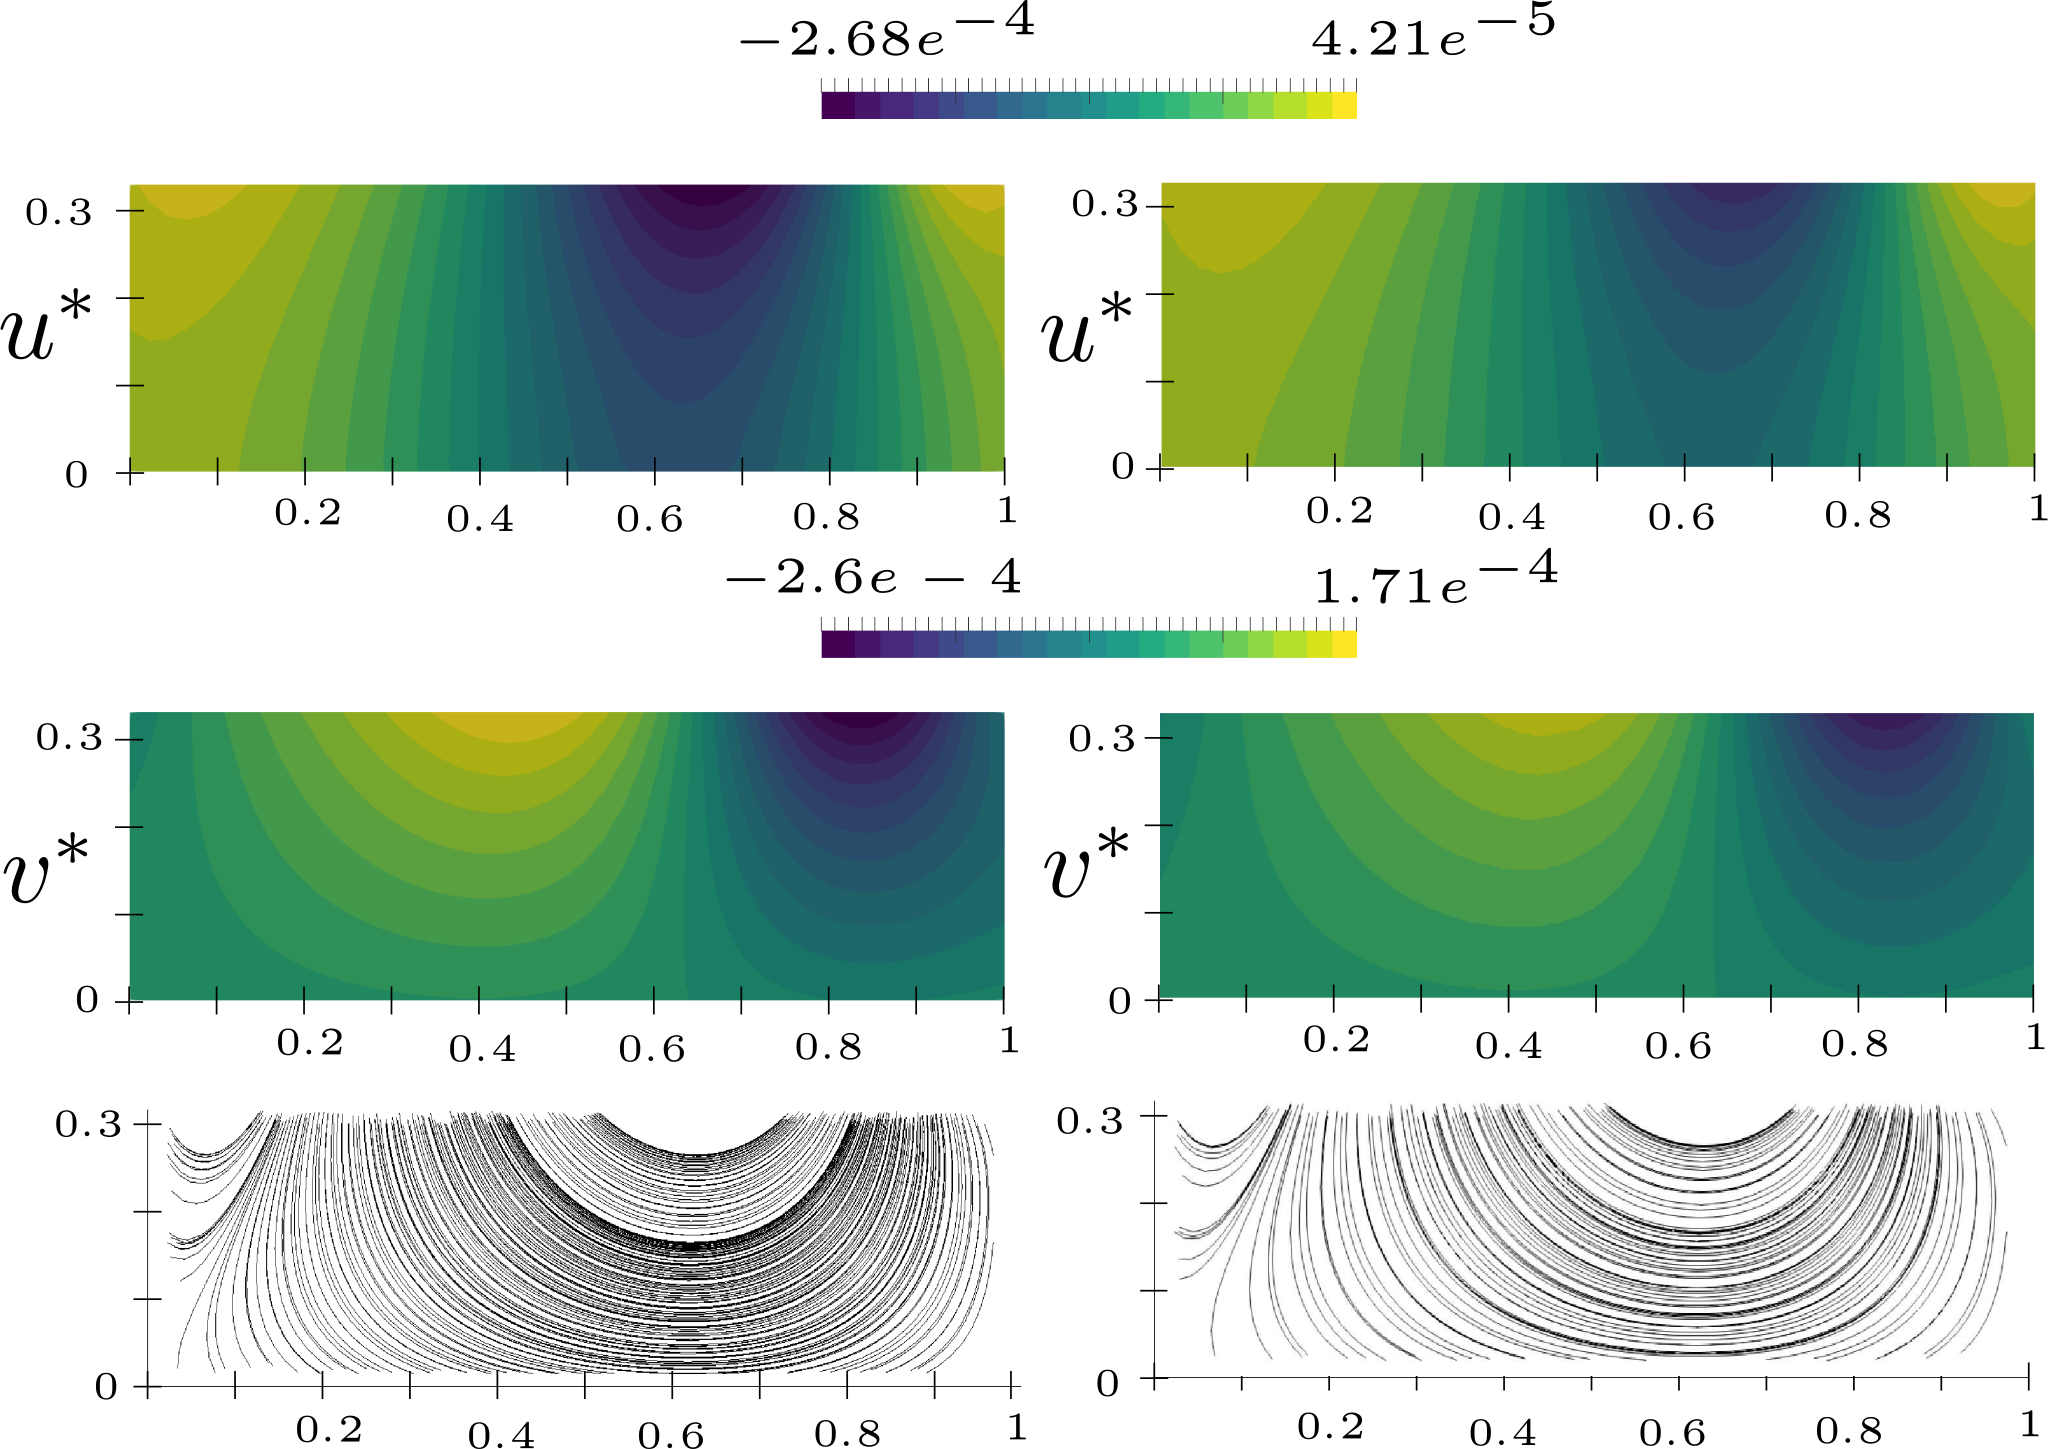
\includegraphics[width=1\linewidth]{chapter_5/figure/re100/vans_u}
	\caption{Left: VANS approach. Right: Homogenized DNS approach. The figure show, from top to bottom, the horizontal velocity the vertical velocity and the streamlines inside the porous domain $\Omega_p$}
	\label{fig:100_u}
\end{figure}

The DNS approach is used as reference case for the comparison. At Reynolds number equal to $100$ we have a fair agreement in the velocities and pressure gradients fields. The contours and the location of the local minima and maxima are the same for the two approaches. If we look at the numerical values, for some fields the relative errors are not negligible however, they are always below $10\%$.
In any case some differences between the two models has to expected since in the VANS approach the micro-scale flow behavior is modeled and of course some of the details that the full DNS is able to retain are lost in the macroscopic approach. 

\begin{figure}[h]
	\centering
	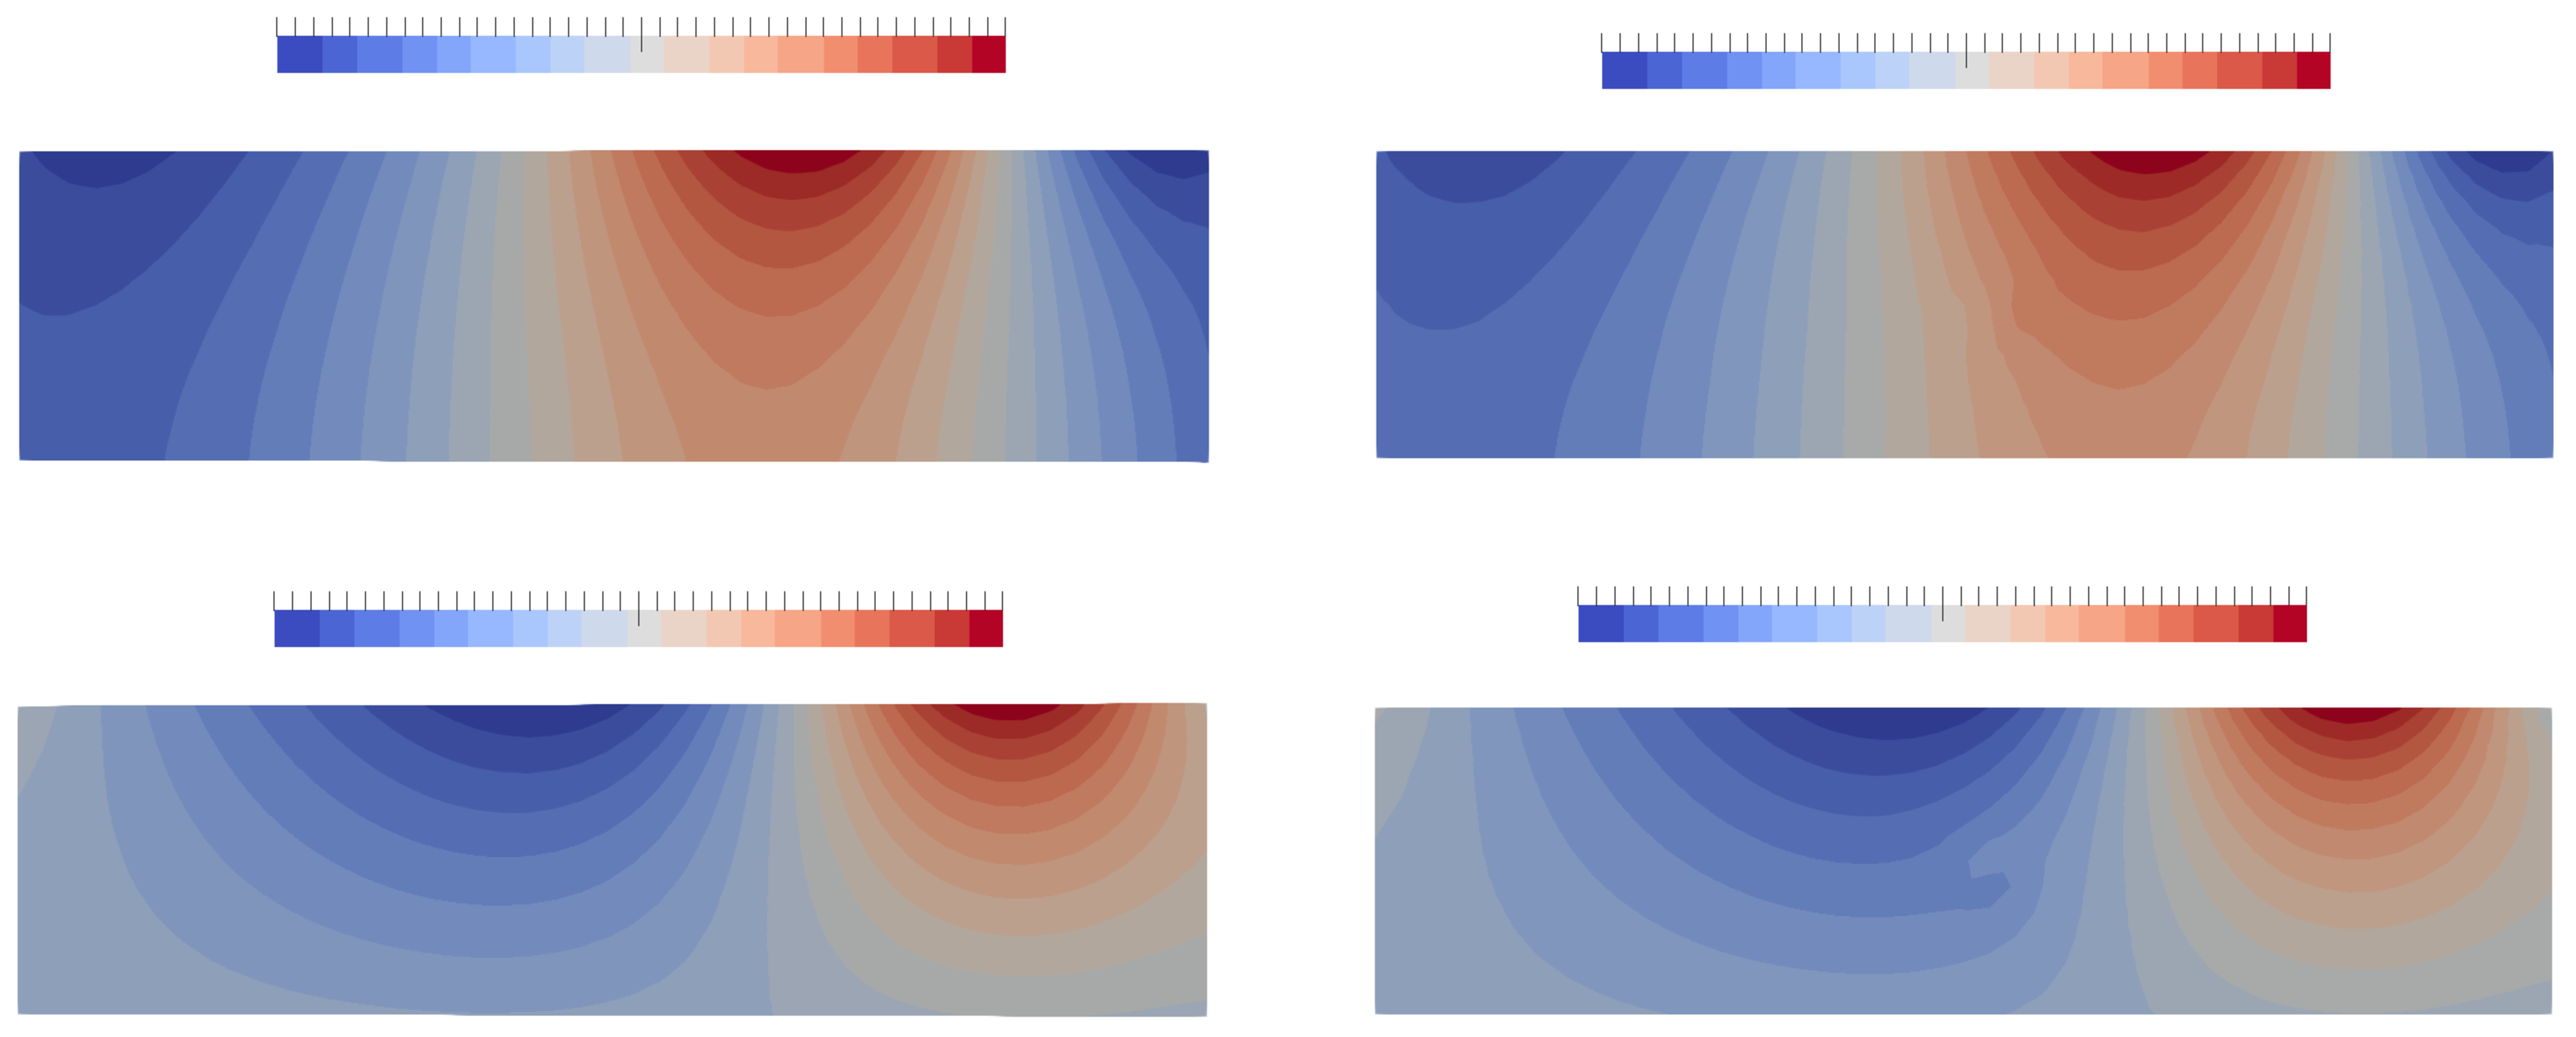
\includegraphics[width=1\linewidth]{chapter_5/figure/re100/vans_p}
	\caption{Left: VANS approach. Right: Homogenized DNS approach. The figure show, from top to bottom, the horizontal and the vertical component of the pressure gradient inside the porous domain $\Omega_p$}
	\label{fig:100_p}
\end{figure}


\subsection{Cavity $Re=1000$ comparison}

The same case and comparison has been done also for a Reynolds number equal to $Re=1000$.
For this case we can confirm the same conclusion as the previous one. Some of the relative errors are even smaller compared to the lower Reynolds number case, this confirm that the model is robust in this range of Reynolds number.

\begin{figure}[h]
	\centering
	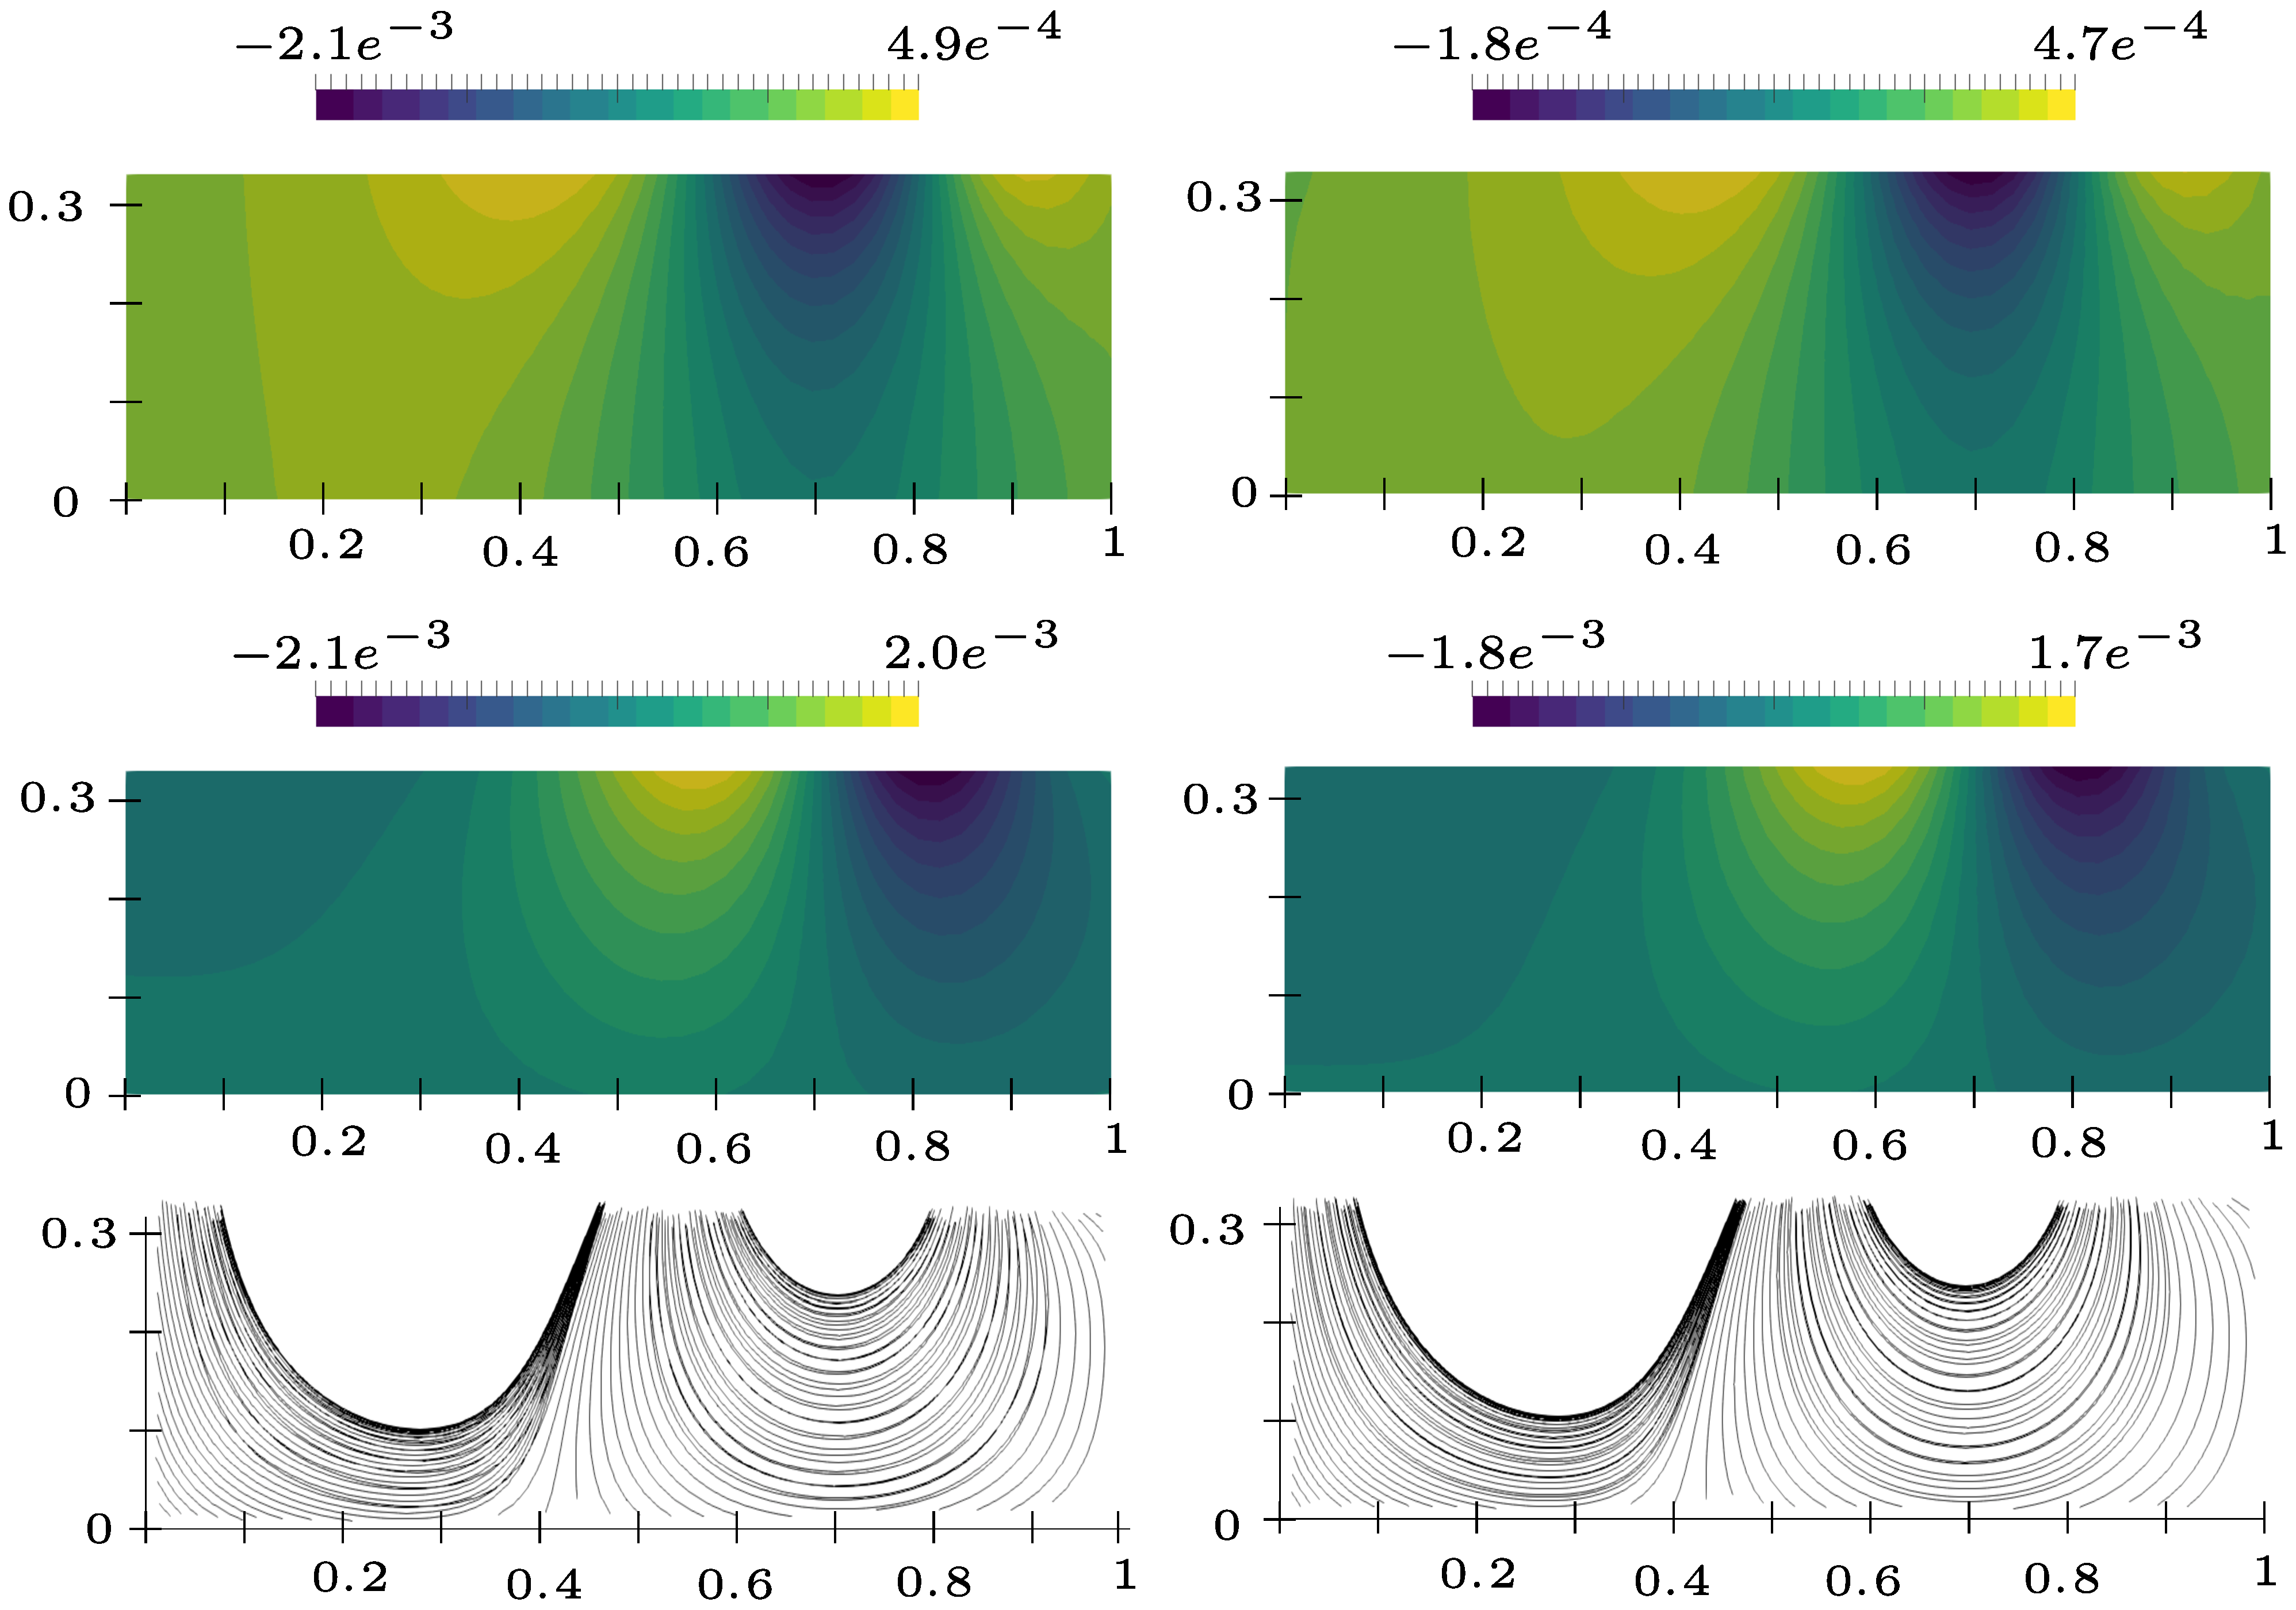
\includegraphics[width=1\linewidth]{chapter_5/figure/re1000/vans_u}
	\caption{Left: VANS approach. Right: Homogenized DNS approach. The figure show, from top to bottom, the horizontal velocity the vertical velocity and the streamlines inside the porous domain $\Omega_p$}
	\label{fig:1000_u}
\end{figure}

\begin{figure}[h]
	\centering
	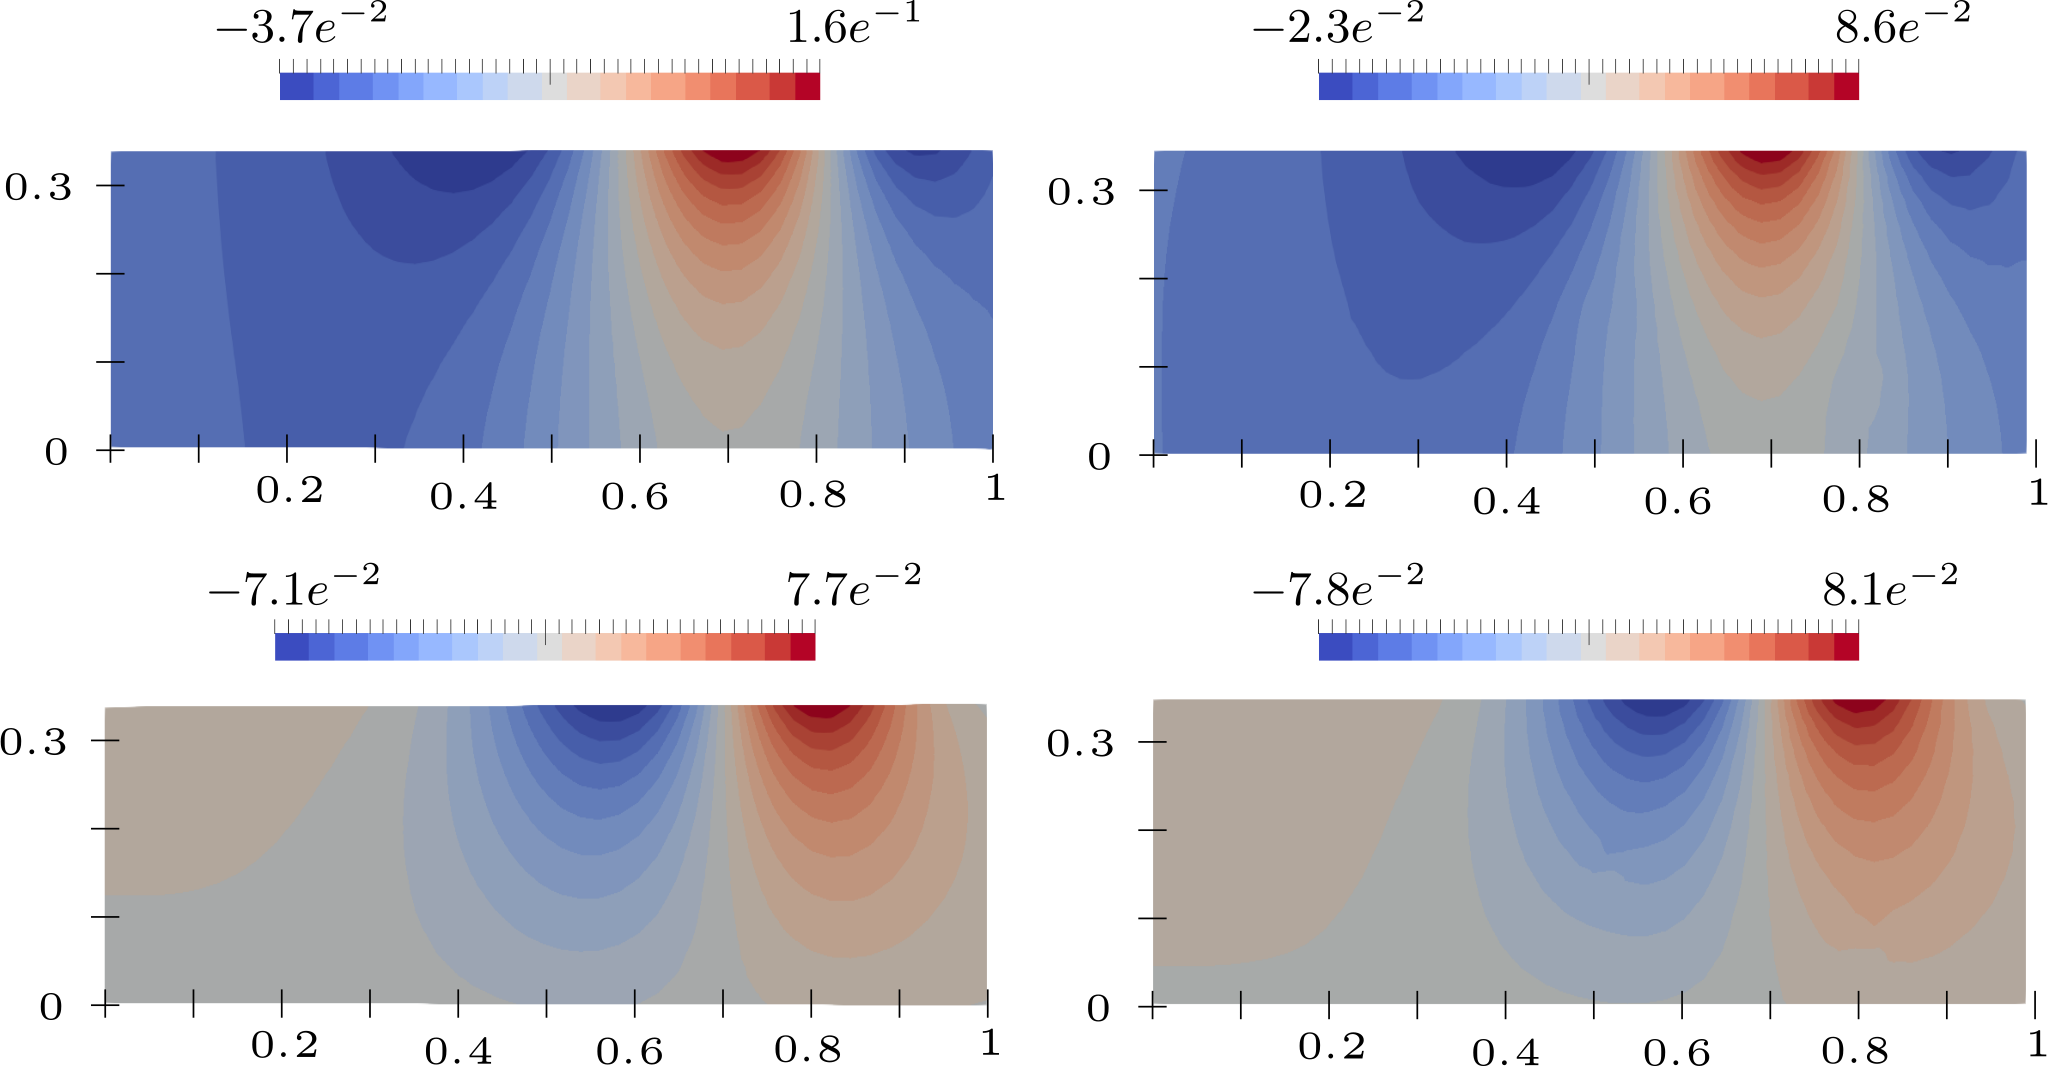
\includegraphics[width=1\linewidth]{chapter_5/figure/re1000/vans_p}
	\caption{Left: VANS approach. Right: Homogenized DNS approach. The figure show, from top to bottom, the horizontal and the vertical component of the pressure gradient inside the porous domain $\Omega_p$}
	\label{fig:1000_p}
\end{figure}


\subsection{Cavity $Re=7000$ using $\mathbf{H}$ metamodel}



\section{Separated flow between hills}
In order to test the effectiveness of the porous media layer to reduce separation we have chose to tho solve the flow over periodically arranged hills. This problesm  has been already investigated experimentally and numerically and is a classical CFD bencmark problem now standardized by the ERCOFTAC. 
The flow experience separation caused by the curved surface of the hill and also recirculation and natural reattachment. The flow is supposed to be periodic and two dimensional, at the Reynolds number tested. Noumerous DNS and LES works can be found in literature with Reynolds numbers up to 10000 (\citet{chang2014simulations}, \citet{breuer2005issues}, \citet{breuer2009flow}, \cite{almeida1993wake} and \cite{temmerman2001large}).
This test case has been studied with two two main objectives, either the modeling and simulation issue or the physical issue. Regarding the first, it is used as a benchmark case to investigate the ability of DNS, RANS and LES to resolve separation from a curved geometry. Furthermore, the flow is also an interesting case to study the physical mechanisms of separation on curved surfaces in more detail.
In our case we have tested smaller Reynolds number in the laminar regime. Although the problem has been chosen especially for the possibility to future extend the study in higher Reynolds number since a lot of data can be found in literature.

\subsubsection{Geometry and condition}
The geometry of the problem is depicted in figure \ref{fig:dom}. The geometry used is the 2D version of the problem since the flow is practically two dimensional in the Reynolds number considered. The dimension of the hill crest and extensions are also showed in the same pictures in their adimensinalized version. However, in our case the heigth of the crest is equal to 1 so the adimensional and dimensional coordinates are the same. The dimensions of the domain are: $L_x = 9.0 h$, $L_y = 3.036 h$ and $L_z = 4.5 h$ where $h$ denotes the hill height and $x,y,z$ are the streamwise, wall-normal and spanwise direction, respectively. It consists of a single streamwise periodic segment and thus covers solely one complete hill with an upstream and a downstream region. In the predictions reported here the domain starts and ends at the hill crest. 
Between one hill and the next one there is a flat plate region of extension $5h$. The pressure induced separation takes place from the first hill curved surface and reattachment is observed at the flat plate part between the two hills.

\begin{figure}[h]
	\centering
	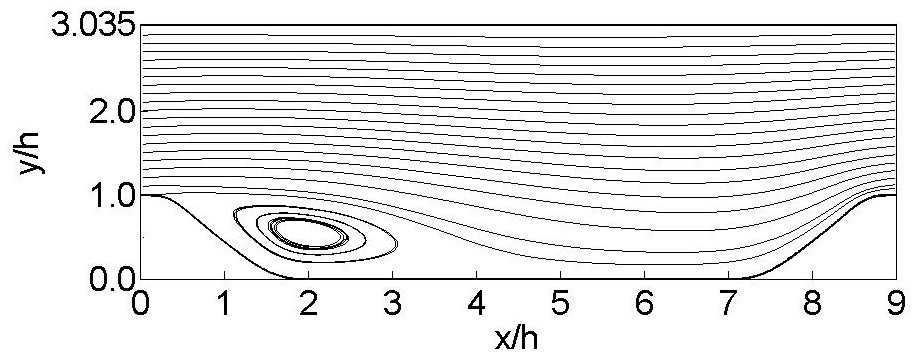
\includegraphics[width=0.7\linewidth]{chapter_5/figure/domain}
	\caption{Domain of the problem with an example of the generic streamlines pattern of the mean flow.}
	\label{fig:dom}
\end{figure}

The problem is discretized using the finite volume method and the mesh used is showed in figure \ref{fig:mesh_hill}. The mesh is purely made of exahedral cell and counts 25000 elements in the two dimensional version. It is possible to download it at \url{https://turbmodels.larc.nasa.gov/Other_LES_Data/2dhill_periodic.html}. The resolution has been already validate in DNS and LES computations so it has not been further investigated here.

\begin{figure}[h]
	\centering
	\includegraphics[width=1\linewidth]{chapter_5/figure/mesh}
	\caption{Mesh used to discretize the problem. On the right side there is an enlargement of the zone on the hill curvature.}
	\label{fig:mesh_hill}
\end{figure}


The inlet and the outlet patches are connected with a periodic boundary condition, at the hill and flat plate surface the no-slip condition is imposed and finally at the top of the domain a slip condition is used.





\subsection{Comparison between smooth and porous leeward side of the hill}

The equation solved are a slightly modified version of the VANS system \eqref{eq:vans_cav} in which the constant macroscopic pressure gradient is introduced as a source term in the momentum.
The non-periodic behavior of the pressure distribution can be accounted for by adding the mean pressure gradient as a source term to the momentum equation in streamwise direction.

\begin{eqnarray}
\begin{cases}
\derp{\vbms}{t} + \dfrac{1}{\varepsilon} \nabla \cdot \left[  \vbmi  \vbmi \right] = -\dfrac{1}{\rho_{\beta}} \nabla \meani{\pb} + \nub \nabla^2 \vbmi \\ 
\qquad \qquad \qquad \qquad \qquad \qquad- \nub \varepsilon \mathbf{H}^{-1} \vbmi +\dfrac{\nub}{\varepsilon} \nabla \varepsilon \cdot \nabla \vbmi + \dfrac{\nub}{\varepsilon} \vbmi \nabla^2 \varepsilon - \mathbf{g}\\
\nabla \cdot \left(\varepsilon \vbmi \right) = 0\\
\vbms = 0 \qquad \textrm{at hill wall} \\
\derp{u}{y}=0 \qquad \textrm{at} y = 3.035h\\
\vbms|_{x_1 = 0} = \vbms|_{x_1 = 9h} \\
\pbms|_{x_1 = 0} = \pbms|_{x_1 = 9h} 
\end{cases}
\end{eqnarray}

The flow is driven by the source term $\mathbf{g}$ and the Reynolds number is computed a posteriori in the following manner:
$$
R_e = \dfrac{U_b h}{\nu}
$$
where $U_b$ is the velocity in the top left corner of the domain, just above the first hill.

In the first case we study the the problem in the stable regime ($Re\leq200$). In this case the source term is equal to $\mathbf{g} = (1e^{-9} \quad0 \quad0)$ and it result in a Reynolds number $Re=70$.
The porous media layer is has the same geometry of the one described in \ref{ch:4}, it means a series of cylinders in staggered arrangement. The cylinders are then arranged on top of the leeward side of the hill and they are aligned with the wall normal direction. Although their extension is not uniform, the line that pass through all the cylinders lid describe the Gaussian:
\begin{equation}
	y_{itf}(x) = \dfrac{2.5}{\sqrt{2\pi}} \textrm{exp}\left( -0.5 x^2 \right)
	\label{eq:gaussian}
\end{equation}

The treatment for the porosity is the same as equation \eqref{eq:porsitity_fun} where in this case the $y_{itf}$ id described by the Gaussian function \eqref{eq:gaussian}.
Instead the permeability tensor has a discontinuity through the same interface line.

The porosity field is depicted in figure \ref{fig:por_gauss}. Where the porosity deep inside the medium, showed in blue, is equal to $0.8$ and the exterior is obviously equal to $1$ and is showed yellow.

\begin{figure}[h]
\centering
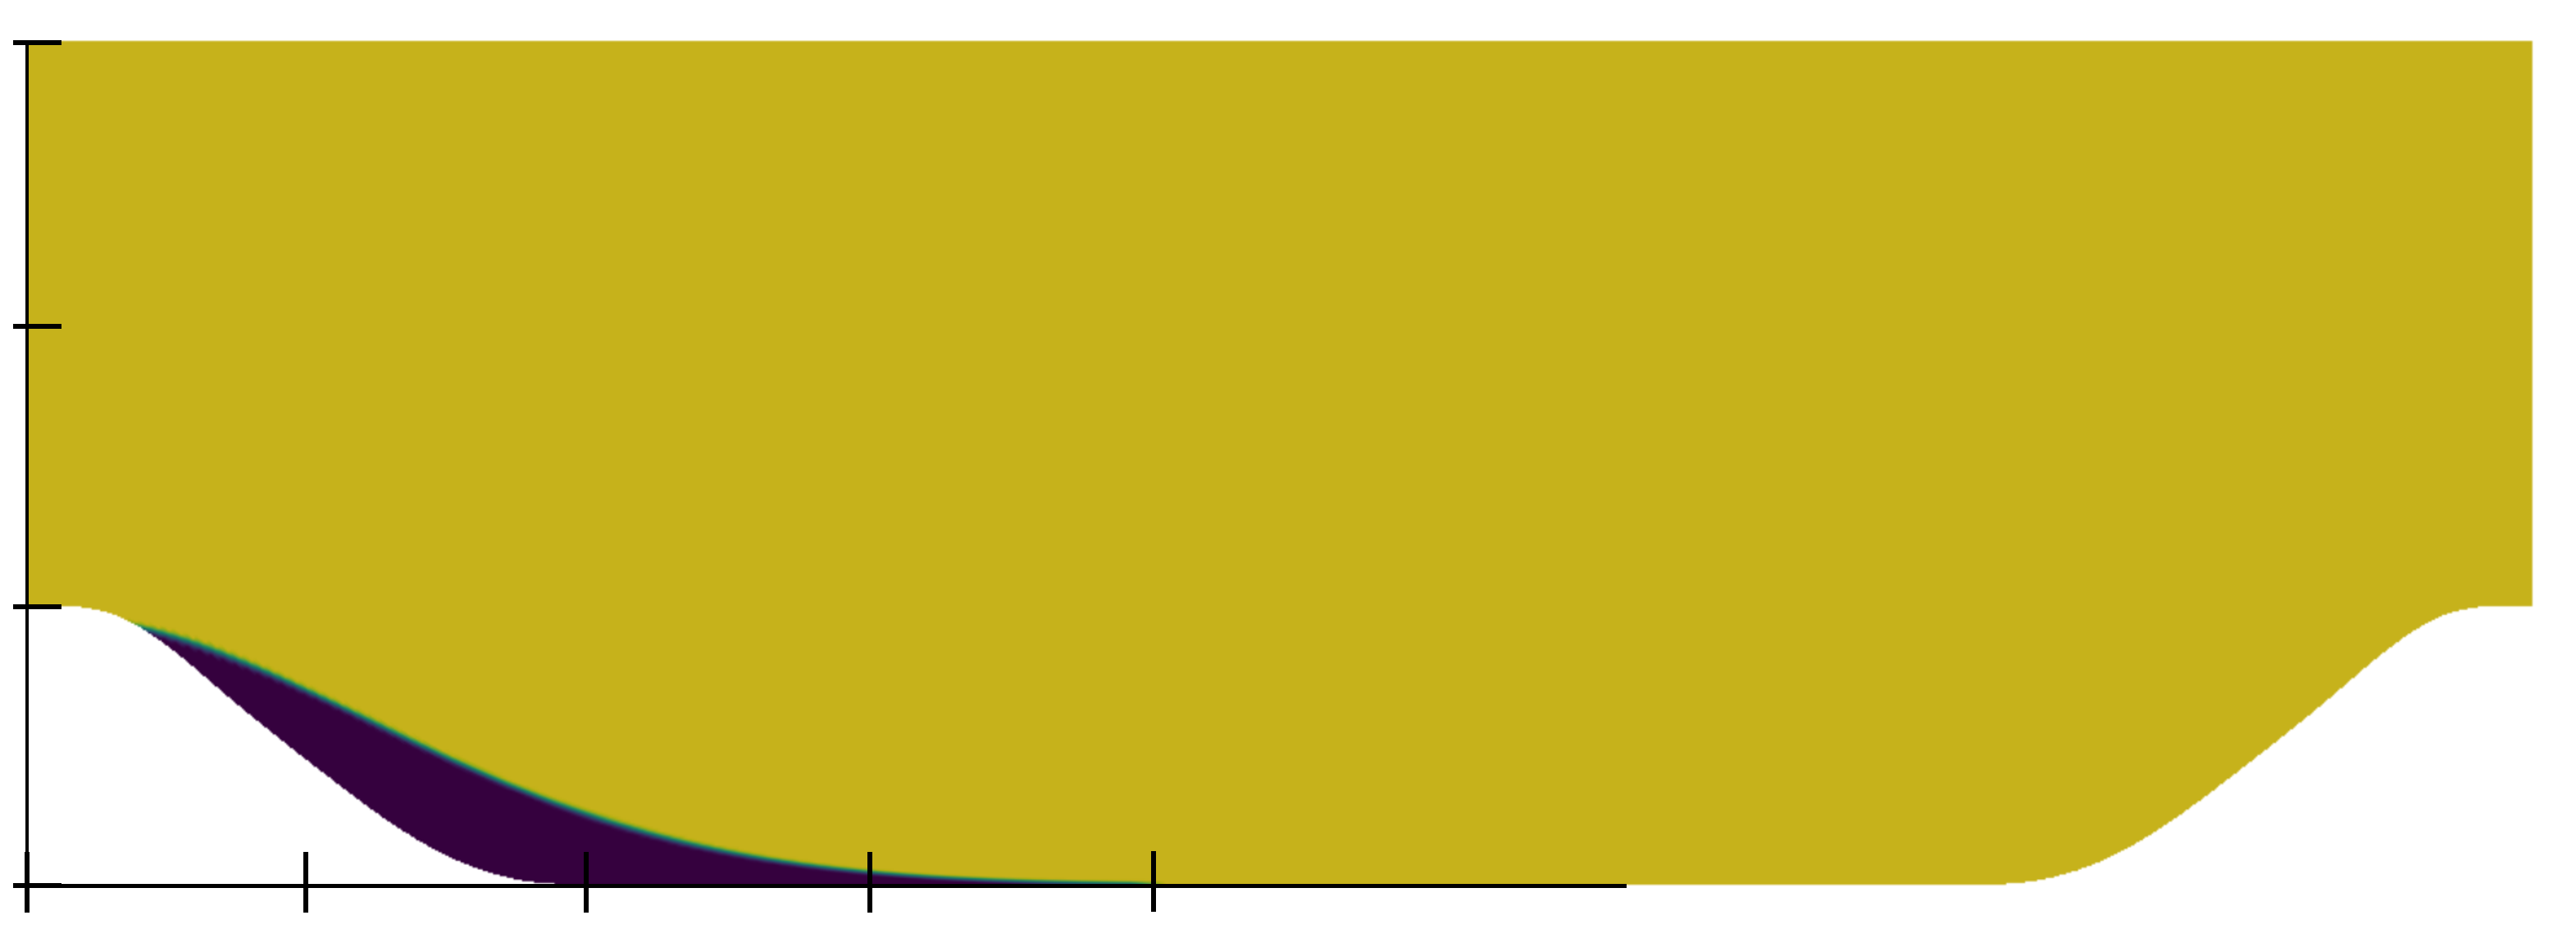
\includegraphics[width=0.7\linewidth]{chapter_5/figure/por}
\caption{Porosity field in the leeward side of the first hill.}
\label{fig:por_gauss}
\end{figure}





\subsection{Comparison in unstable regime}



\section{Conclusions}

If it would be possible to obtain systematically the same results with a reduced information model \footnote{like a general metamodel or a macroscopic model for porous media or a turbulence model for turbulent flow} and a full physic simulation we would be in a paradox. Basically it would means that some of the input information are redundant. This statements should be kept in mind when making analysis on the macroscopic model against the DNS.


